\newpage
\label{sec:appendix}
\section{Our StylEx vs Lang et al.'s}
\label{app:A}

\begin{figure}[h]
    \centering
    \subfloat[TensorFlow (theirs)]{
         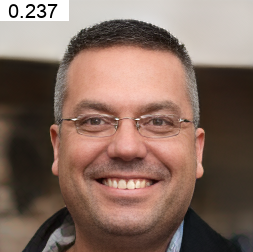
\includegraphics[scale=0.4]{images/StylEx_theirs.PNG}
         \label{fig:TensorFlow classifier}}
     \subfloat[PyTorch (ours)]{
         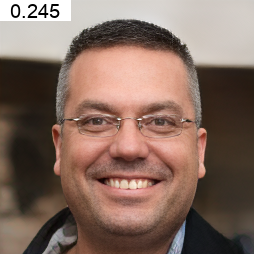
\includegraphics[scale=0.4]{images/StylEx_ours.PNG}
         \label{fig:PyTorch classifier}}
  \caption{\centering \textbf{Comparison of StylEx models results.} The probabilities shown correspond to being classifier as young.}
  \label{fig:PyTorch vs TensorFlow classifier}
\end{figure}

\begin{figure}[h]
    \centering
    \subfloat[Original image]{
         \includegraphics[scale=0.3]{images/69931_256.png}
         \label{fig:TensorFlow classifier2}}
    \subfloat[TensorFlow (theirs)]{
         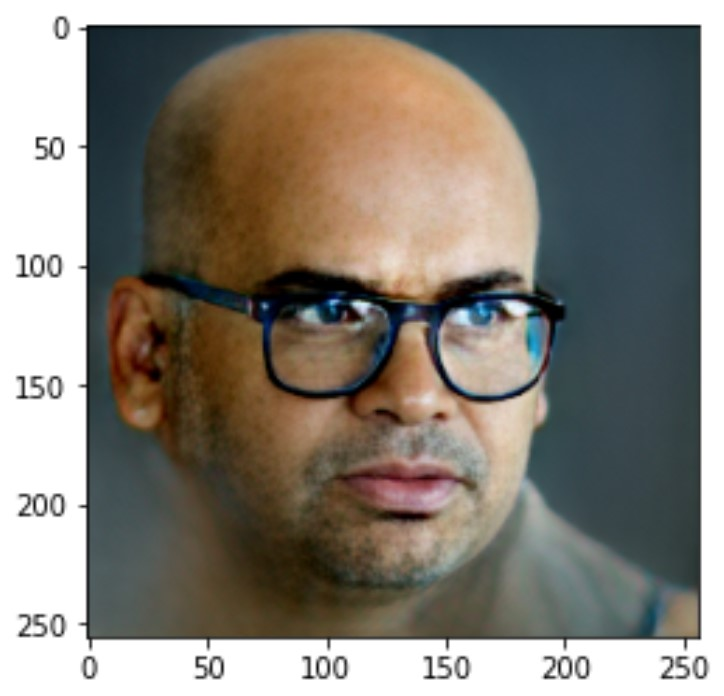
\includegraphics[scale=0.3]{images/encoded_image_theirs.jpeg}
         \label{fig:TensorFlow classifier3}}
     \subfloat[PyTorch (ours)]{
         \includegraphics[scale=0.31]{images/encoded_image_our.png}
         \label{fig:PyTorch classifier2}}
  \caption{\centering \textbf{Comparison of StylEx models encoding and then reconstructing an image.} Both models use their encoder and classifier to produce the latent variable. Then using their generator the image is reconstructed from the latent variable.}
  \label{fig:PyTorch vs TensorFlow encoder}
\end{figure}

\section{AttFind Lang et al.'s top attributes}
\label{app:B}
\begin{figure}[H]
\centering
    \subfloat[\centering \small \textbf{Attribute 1}  "Skin Pigmentation"]{       \includegraphics[width=0.23\textwidth]{images/1_skin_pigmentation_theirs.png}}%\label{fig:att2}}
    \hspace{0.2em}
    \subfloat[\centering \small \textbf{Attribute 2}  "Eyebrow Thickness"]{
        \includegraphics[width=0.23\textwidth]{images/2_eyebrow_thickness_theirs.png}}%\label{fig:att2}}
    \hspace{0.2em}
    % \hfill
    \subfloat[\centering \small \textbf{Attribute 3}  "Add/Remove Glasses"]{
        \includegraphics[width=0.23\textwidth]{images/3_glasses_theirs.png}}%\label{fig:att3}}
    \hspace{0.2em}
    \subfloat[\centering \small \textbf{Attribute 4}  "Dark/White Hair"]{
        \includegraphics[width=0.23\textwidth]{images/4_hair_theirs.png}}%\label{fig:att4}}
    
    
    \caption {\textbf{Top 4 attributes for the perceived age classifier detected by Lang et al.'s pre-trained model.} These images show how the probability of classifying a person as young or old changes based on each attribute. On the first column of each image, we display the probability of the person being classified as old and on the second column the probability of them being classified as young.} 
    \label{fig:top 4 attrs theirs}
\end{figure}

\section{Hyperparameters} \label{app:hyperparameters}
\begin{table}[H]
\centering
\begin{tabular}{l|c|c}
\hline
                                                                                                       & Our StylEx  & Lang et al's StylEx   \\ \hline \hline
Step Size                                                                                              & 1e-3        & 2e-4                  \\ 
Number of Steps                                                                                        & 50,000      & 250,000               \\ 
\begin{tabular}[c]{@{}l@{}}Total Loss Weights\\ ($\mathcal{L}_{rec}$, $\mathcal{L}_{adv}$, $\mathcal{L}_{c}$, $\mathcal{L}_{PL}$) \end{tabular} & 1,1,1,1     & 1,1,1,?               \\ 
\begin{tabular}[c]{@{}l@{}}Reconstruction Loss Weights \\ ($\mathcal{L}_{w}$, $\mathcal{L}_{x}$, $\mathcal{L}_{LPIPS}$)\end{tabular}                                  & .1, 1, .1   & .1, 1, .1             \\ 
Latent Dimension                                                                                       & 32          & 512                   \\ 
Number of Classes                                                                                      & 2           & 2 (depending on data) \\ 
Image Resolution                                                                                       & 32          & 256                   \\ 
Classifier Structure                                                                                   & DenseNet121 & MobileNet             \\ 
Optimizer                                                                                              & Adam        & ?                     \\ 
\end{tabular}
\vspace{0.5cm}
\caption{Training hyperparameters}
\label{tab:hyperparameters}
\end{table}
\normalsize

\section{MNIST Reconstruction}
\label{app:MNIST_Reconstruct}
\begin{figure}[H]
    \centering
    \begin{subfigure}[]{0.3\textwidth}
         \centering
         \includegraphics[width=\textwidth]{images/Original Image.png}
         \caption{Original image}
         \label{fig:y equals x}
     \end{subfigure}
     \hspace{10pt}
     \begin{subfigure}[]{0.3\textwidth}
         \centering
         \includegraphics[width=\textwidth]{images/Reconstruction.png}
         \caption{Reconstructed image}
     \end{subfigure}
    \caption{An example of image reconstruction on the MNIST dataset. The StylEx had converged however, it was trained conditioned on a classifier that always predicted 8, thus was effectively trained without a classifier. It's loss curves can be found { \href{https://app.labml.ai/run/841a8fde81b511eca9da0242ac1c0002}{here}}.}
    \label{fig:MNIST_Reconstruct}
\end{figure}

\section{Verbal Description Study} \label{app:classificationstudy}
\begin{table}[H]
\begin{minipage}{.8\linewidth}
{\begin{tabular}{m{1.5cm}|m{1.5cm}|m{2.4cm}|m{2.4cm}|m{2.4cm}}
\hline
\multicolumn{5}{c}{Cats/Dogs Classifier}                                                                                                   \\ \hline \hline
\includegraphics[width=1.5cm]{images/Screenshot from 2022-02-02 21-11-31.png} & {\includegraphics[width=1.5cm]{images/Screenshot from 2022-02-02 21-11-16.png}} & {eye:  0.73}   & {pupil: 0.16} & shape: 0.1   \\
\includegraphics[width=1.5cm]{images/Screenshot from 2022-02-02 21-11-49.png} & \includegraphics[width=1.5cm]{images/Screenshot from 2022-02-02 21-12-07.png} & {mouth: 0.73} & {open: 0.3}   & tongue: 0.16 \\
{\includegraphics[width=1.5cm]{images/Screenshot from 2022-02-02 21-12-23.png}} & {\includegraphics[width=1.5cm]{images/Screenshot from 2022-02-02 21-12-34.png}} & {ear:  0.90}     & {right: 0.06}    & become: 0.06   
\end{tabular}}
\caption*{(a)}
\end{minipage}
\begin{minipage}{.8\linewidth}
{\begin{tabular}{m{1.5cm}|m{1.5cm}|m{2.4cm}|m{2.4cm}|m{2.4cm}}
\hline
\multicolumn{5}{c}{Face (age/gender) Classifier}                                                                                                        \\ \hline \hline
\includegraphics[width=1.5cm]{images/Screenshot from 2022-02-02 22-41-05.png} & {\includegraphics[width=1.5cm]{images/Screenshot from 2022-02-02 22-41-19.png}} & {eyebrow: 0.90} & {thick: 0.17} & brow: 0.07 \\
\includegraphics[width=1.5cm]{images/Screenshot from 2022-02-02 22-41-35.png} & \includegraphics[width=1.5cm]{images/Screenshot from 2022-02-02 22-41-47.png} & {tooth: 0.30} & {lip:  0.10} & disappear: 0.07 \\
\includegraphics[width=1.5cm]{images/Screenshot from 2022-02-02 22-42-03.png} & \includegraphics[width=1.5cm]{images/Screenshot from 2022-02-02 22-42-15.png} & {glass: 0.90} & {size: 0.13} & bigger: 0.10    \\
\includegraphics[width=1.5cm]{images/Screenshot from 2022-02-02 22-42-29.png} & \includegraphics[width=1.5cm]{images/Screenshot from 2022-02-02 22-42-42.png} & {mouth: 0.70} & {open: 0.40} & lip:  0.10       \\
\includegraphics[width=1.5cm]{images/Screenshot from 2022-02-02 22-42-54.png} & \includegraphics[width=1.5cm]{images/Screenshot from 2022-02-02 22-43-04.png} & {bright: 0.37} & {skin: 0.30} & light: 0.27     \\
\includegraphics[width=1.5cm]{images/Screenshot from 2022-02-02 22-43-13.png} & \includegraphics[width=1.5cm]{images/Screenshot from 2022-02-02 22-43-30.png} & {mustache: 0.93} & {facial: 0.07} & hair: 0.07      \\
\includegraphics[width=1.5cm]{images/Screenshot from 2022-02-02 22-43-44.png} & \includegraphics[width=1.5cm]{images/Screenshot from 2022-02-02 22-43-55.png} & {eye:  0.77} & {color: 0.47} & eyelash: 0.13  
\end{tabular}}
\caption*{(b)}
\end{minipage}
\caption{\textbf{Verbal description study results.} The 3 most common words used in user descriptions for the Cat/Dogs (a) and Face (age/gender) (b) classifiers. This user study proves the distinctness of each attribute since the most common word used to describe each attribute change is different per classifier.}
\label{tab:top3}
\end{table}

